\chapter{Einleitung}

\textit{Umgang mit grammatikalischen Geschlechtern: Aus Gründen der Spracheleganz wird vor allem die männliche Form (zum Beispiel "`Benutzer"') verwendet. Die weibliche Form ist jedoch sinngemäss mitgemeint.}

\section{Bedeutung  und Zweck von Diagrammen}

Im Informationszeitalter sind Daten von grosser Bedeutung, der Datenfluss vergrössert sich ständig. Um Daten darstellen zu können, müssen sie zuerst gesammelt, sortiert und formatiert werden, bevor mit der Auswertung begonnen werden kann. Das Sammeln von Daten stellt oftmals keine besondere Schwierigkeit dar, das Auswerten, Darstellen und Interpretieren ist eine Herausforderung.

Die graphische Darstellung von Daten, das Diagramm, ist von grosser Bedeutung für die Gesellschaft. Man findet Diagramme überall: In etlichen Wissenschaften, wo sie nicht wegzudenken sind, in der Industrie, in Zeitungen, in Werbungen.

% kann man das gleiche zitat wie im visualisierungs buch hinzufügen?

Das Ziel eines Diagramms ist die visuelle Repräsentation einer gegebenen Datenmenge, um damit eine effiziente Auswertung zu ermöglichen. Die Analyse, das Verständnis und die Kommunikation sollen erleichtert werden \cite[Kapitel 1.1]{viz}. Der Leser sollte sich mit der Datenmenge auseinandersetzen können, ohne die Rohdaten selbst betrachten zu müssen. Je nachdem wie das Diagramm graphisch umgesetzt wird, können verschiedene Zusammenhänge und Informationen des Datensatzes hervorgehoben oder in den Hintergrund gestellt werden, was einen Einfluss auf die Vermittlung hat. 
Das Ziel eines Diagramms ist es jedoch, die Datenmenge möglichst unverfälscht darzustellen \cite[Kapitel 1.1]{viz}. 



% kann man direkt aus visualisationsbuch abschreiben, dann aber nur die quelle angeben, die im buch verwiesen ist?

Konventionell werden Diagramme in Zeitungen, Artikeln abgedruckt. Der Autor trifft Entscheidungen, wie die Daten in graphischer Form dargestellt werden und erstellt auf Basis dieser ein Diagramm. Nach dem Druck kann es vom Leser betrachtet werden, jedoch kann dieser die Darstellung nicht mehr verändern, das Diagramm ist statisch. Er hat darum keinen Einfluss, wie die Daten in diesem \textit{statischen Diagramm} dargestellt und an ihn vermittelt werden.

Durch das Aufkommen von modernen Computern und Smartphones haben sich die Möglichkeiten zur Darstellung erweitert: Dem Benutzer ist es möglich, mit dem Diagramm zu interagieren. Diese Maturaarbeit wurde vom Artikel \textit{The Eyes Have It: A Task by Data Type for Information Visualizations} von B. Shneiderman \cite{shneiderman} inspiriert. Der Artikel untersucht, wie ein Benutzer eine Programmoberfläche wahrnimmt und auf welche Weise er mit ihr interagiert. Auch beschreibt der Artikel, wie die Oberfläche aufgebaut sein sollte, damit der Benutzer sich im Programm orientieren kann, die Programmlogik versteht und ohne grossen Aufwand bedienen kann. Im Artikel stellt \citeauthor{shneiderman} zudem das \textit{Mantra der Informationssuche (Information-Seeking Mantra)} auf, das beschreibt, wie der Benutzer typischerweise mit einer Oberfläche interagiert: Überblick zuerst, Zoomen und Filtern, als Letztes Details auf Abruf \cite{shneiderman}.

Man findet unter anderem in Online-Zeitschriften solche \textit{dynamischen Diagramme}, welche Daten darstellen, die für den Artikel relevant sind und interaktiv vom Benutzer bedient werden können. Die Abbildungen \ref{fig:nytimes-taxes} und \ref{fig:nytimes-realestate} demonstrieren, wie das Potential der Interaktion auf eine interessante Weise ausgenutzt werden kann.

In der Abbildung \ref{fig:nytimes-taxes} ist ein Blasendiagramm dargestellt. Jede Blase stellt eine Firma dar, je nach Börsenwert ist die Blase unterschiedlich gross. Die Firmen sind in horizontaler Richtung nach ihrem Steuertarif geordnet, die verschiedenen Farben stellen die jeweilige Industrie, in der die Firma tätig ist, dar. Wenn die Maus über die Blase fährt, wird ein \textit{Popup} sichtbar, das weitere Informationen zur Firma anzeigt wie der exakte Steuertarif, die absolute Menge an Steuern, die bezahlt wurde oder der Umsatz der Firma.

\begin{figure}[H]
	\centering
	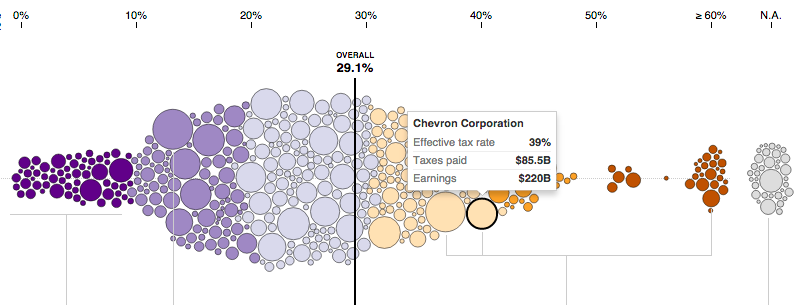
\includegraphics[width=\linewidth]{images/nytimes-taxes-zugeschnitten}
	\caption[Blasendiagramm in The New York Times (\citedate{nytimes-taxes})]{Ein Blasendiagramm, das Steuerabgaben und Steuersätze von US-Firmen darstellt. \cite{nytimes-taxes}}
	\label{fig:nytimes-taxes}
\end{figure}

Die Webseite in Abbildung \ref{fig:nytimes-realestate} berechnet anhand von vom Benutzer festgelegten Faktoren, ob der Kauf eines Hauses profitabler wäre als die Miete. Es sind Faktoren vorhanden wie der Zinssatz, die Entwicklung der Miete und der Wert des Hauses, der Steuersatz für Grundstücke, die Inflationsrate. Die verschiedenen Faktoren kann der Benutzer durch einen \textit{Regler} anpassen. Dabei kann er durch die Höhe der Balken über dem Regler sehen, wie sich der Faktor auf das Resultat auswirkt (ob der Kauf oder die Miete profitabler wäre). Beim verschieben des Reglers wird das Ergebnis automatisch aktualisiert, so sieht der Benutzer den Zusammenhang der Faktoren und der Berechnung.

\begin{figure}[H]
	\centering
	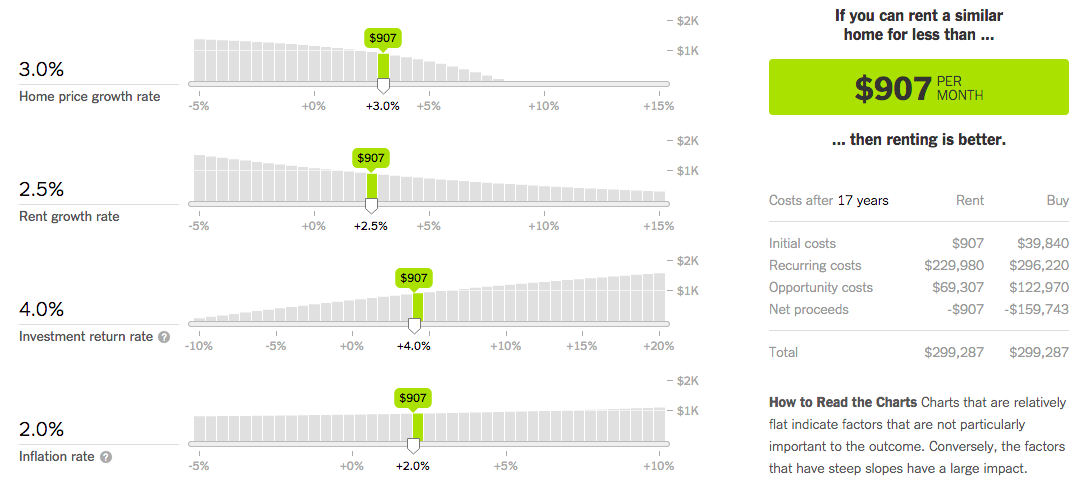
\includegraphics[width=\linewidth]{images/nytimes-realestate-zugeschnitten}
	\caption[Interaktives Diagramm in The New York Times (\citedate{nytimes-realestate})]{Interaktives Diagramm mit verstellbaren Reglern, das die Profitabilität des Kaufs eines Hauses darstellt. \cite{nytimes-realestate}}
	\label{fig:nytimes-realestate}
\end{figure}

%beispiele aus ingenieurbereich?

An den Diagrammen in Abbildung \ref{fig:nytimes-taxes} und \ref{fig:nytimes-realestate} kann man den Vorteil von dynamischen Diagrammen gut demonstrieren: In Abbildung \ref{fig:nytimes-taxes} wird der dritte Teil des Mantras der Informationsvisualisierung angewendet, Details auf Abruf: Der Tooltip zeigt zusätzliche Informationen einer angewählten Firma an. Wegen Platzmangel wäre es nicht möglich gewesen, die gesamte Information aller Firmen in einem statischen Diagramm darzustellen.

In Abbildung \ref{fig:nytimes-realestate} verändern sich die einzelnen Diagramme je nach Einstellung der Faktoren. Diese Verhaltensweise ist nicht umzusetzen in einem statischen Diagramm.

Die von \citeauthor{shneiderman} beschriebenen Prinzipien für das Design von Benutzeroberflächen werden in dieser Arbeit berücksichtigt. Es werden interaktive, dynamische Diagramme entwickelt, die den Informationsertrag des Benutzers verbessern sollten. Er sollte sich mit den Daten effizienter auseinandersetzen können, besser verstehen und Spass an der Erkundung des Datensatzes haben \cite[Kapitel 1]{shneiderman}.

\section{Ziel dieser Arbeit}

Das Ziel dieser Arbeit ist die Entwicklung einer eigenen Applikation, die dynamische Diagramme in einem Web-Browser darstellt. Sie soll den Prinzipien von Shneiderman folgen und dem Benutzer erlauben, eine bessere Analyse, ein besseres Verständnis des Datensatzes zu erlangen. Auch soll die Applikation dem Benutzer Spass machen und ihn ermuntern, sich mit dem Diagramm auseinanderzusetzen \cite[Kapitel 1]{shneiderman}.

Das Design der Applikation wird auch aufgezeigt, mit dem diese Diagramme erstellt werden, welche Probleme bei der Entwicklung aufgetreten sind; verwendete Entwicklungswerkzeuge werden vorgestellt.

\section{Wahl des Diagrammtyps für die Applikation}

Es gibt sehr viele Arten von Diagrammen, welche sich jeweils für verschiedene Datenstrukturen eignen. 
% beispiele pie diagramme und so?
Diese Applikation beschränkt sich auf zwei grundlegende Diagrammtypen: Das \textit{Punktdiagramm} und das \textit{Liniendiagramm}.

\begin{figure}[!htbp]
	\centering
	\begin{minipage}{0.45\textwidth}
		\centering
		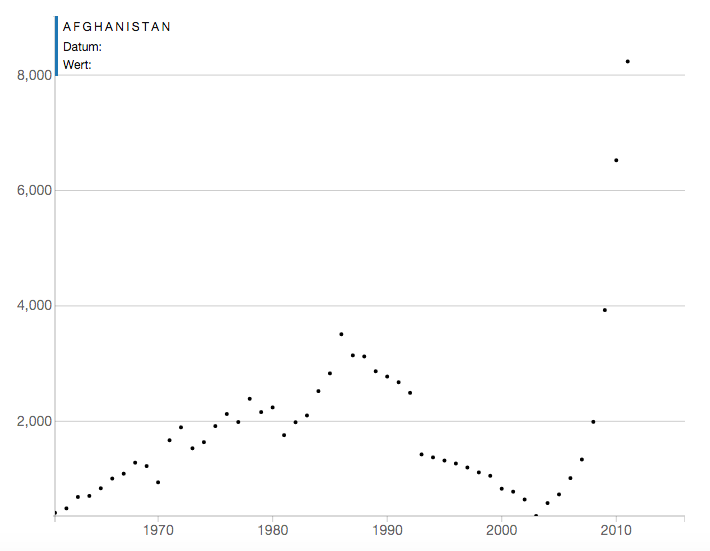
\includegraphics[width=\linewidth]{images/scatterplot_no_interpolation}
	\end{minipage}\hfill
	\begin{minipage}{0.45\textwidth}
		\centering
		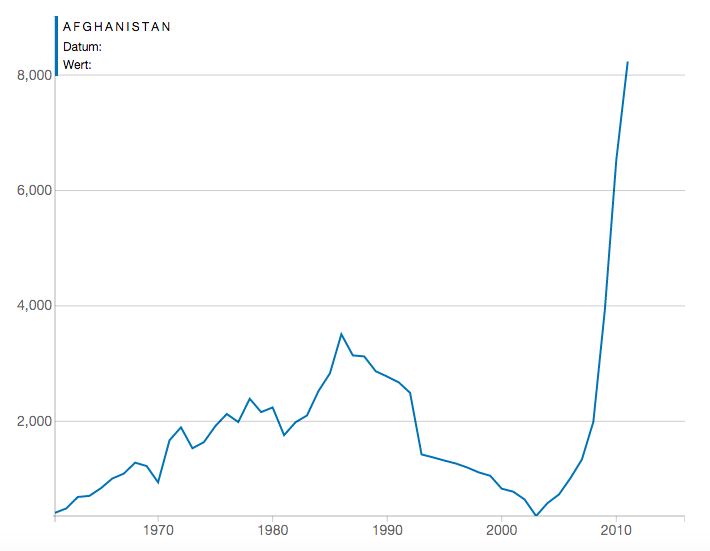
\includegraphics[width=\linewidth]{images/scatterplot_interpolated}
	\end{minipage}
	\caption[Vergleich zwischen Punktdiagramm und Liniendiagramm]{Beispiel von Diagrammen am Datensatz des CO\textsubscript{2}-Ausstosses von Afghanistan. Links: Punktdiagramm. Rechts: Liniendiagramm mit linearer Interpolation.}
	\label{fig:scatterplot}
\end{figure}

Das Punktdiagramm und das Liniendiagramm werden sowohl in der Wissenschaft als auch in den Medien oft verwendet. In diesen Diagrammen werden Skalen in der Ebene oder im Raum festgelegt, die ein Koordinatensystem beschreiben. Mindestens eine Achse dient als Skala der unabhängigen Variablen (der Dimension, die den Beobachtungsraum der Daten aufspannen). Die restlichen Achsen dienen als Skala der abhängigen Variablen, Ausprägungen, die abgetragen werden und mit graphischen Symbolen, wie etwa Kreisen, Kreuzen oder Vierecken, markiert werden \cite[Kapitel 5.2]{viz}. Beim Liniendiagramm werden zusätzlich die benachbarten Punkte durch eine Linie oder einen Kurvenabschnitt verbunden, was Trends und Strukturen der Daten deutlicher darstellt, und Datenpunkte, die durch Linien verbunden sind, werden zusätzlich gruppiert \cite[Kapitel 5.2]{viz}. In der Abbildung \ref{fig:scatterplot} sind ein Punktdiagramm und ein Liniendiagramm dargestellt, die den Verlauf des CO\textsubscript{2}-Ausstosses von Afghanistan darstellen.

\section{Wahl der Programmiersprache für die Applikation}

Interaktive Diagramme werden in der Praxis fast ausschliesslich für den Web-Browser entwickelt, wie auch in dieser Arbeit. Technologien wie HTML, CSS, SVG und JavaScript werden verwendet, sie ermöglichen die dynamische Manipulation durch den Benutzer. Diese Technologien werden durch praktisch alle neueren Smartphones, Tablets, Laptops und Desktops unterstützt.
